\documentclass[a4paper,ngerman]{scrartcl}

\usepackage{amsmath}
\usepackage{amsfonts}
\usepackage{amssymb}
\usepackage[utf8]{inputenc}
\usepackage{graphicx}
\usepackage[ngerman]{babel}
\usepackage{hyperref}
\usepackage{float}
\usepackage{caption}
\usepackage{subcaption}
\usepackage{multirow}  %for tables
\usepackage{icomma} % Handle german comma as decimal point in numbers
\usepackage{units,siunitx} % Write units with correct spacing
\usepackage{upgreek} % provide non-italic greek letters
\usepackage{url}
\usepackage{hepnames}
%\usepackage{subfig}

% Formatting of table & figure captions
\captionsetup{font={sf,footnotesize},labelfont=bf,skip=6pt}
\captionsetup[sub]{font={sf,footnotesize}} % setting for subcaptions
\sisetup{locale = DE, % use "," as decimal point instead of "."
per-mode=reciprocal, % use fractions instead of ^{-1} when doing \si{... \per ...} 
exponent-product={\cdot},% used \cdot in front of 10^x
separate-uncertainty % give out uncertainty with \pm instead of in brackets
} 
\setlength{\abovecaptionskip}{6pt}
\setlength{\belowcaptionskip}{0pt}

\title{Landé-Faktor des Myons\\Versuchsvorbereitung}
\date{\today}
\author{Michel Rausch, Michael Eliachevitch}

\begin{document}

\maketitle
\tableofcontents
\newpage

\section{Einleitung}
\label{sec:einfuhrung}
% Ziel: Bestimmung der Lebensdauer und des Landé-Faktors von Myonen, 
% Myonen sinde Sekundärteilchen der kosmischen Strahlung
% wir werden ständig mit Myonen bombardiert, ohne es zu merken


\section{Theoretische Grundlagen}
\label{sec:theorie}

\subsection{Enstehung von Myonen in Luftschauern}
\label{sec:luftschauer}

Die Erde wird ständig hochenergetischer kosmischer Strahlung getroffen. 
Diese besteht zu einem Großteil von 85\% aus Protonen, aber auch aus 12\% $alpha$-Teilchen und etwa 2\% schweren Kernen,
sowie einer elektromagnetischen Komponente mit Elektronen und Gammaquanten~\ref{ref:bb}.
Aus Experimenten ist bekannt, dass die kosmische Strahlung ein Potenzspektrum der Form

\begin{equation}
  N(> E) = K \cdot \left(\frac{E}{E_0}\right)^{-\gamma}
  \label{eq:powerlaw}
\end{equation}
hat, mit $E_0 = \SI{e16}{eV}$, $K = \SI{3e4}{\per\square\meter\per\hour}$ und dem Exponenten $\gamma$ in einem Bereich zwischen 1,7 und 2,1.
Wenn man das Spektrum doppelt logarithmisch aufträgt, erhält man eine Gerade mit einer dem Faktor $\gamma$ entsprechenden Steigung.
Bei $\SI{4e15}{eV}$ wird $gamma$ etwas größer, was als "`Knie"' bezeichnet wird, und etwa $\SI{e18}{eV}$ wird der Faktor $gamma$ wieder etwas kleiner, was als "`Knöchel"' bezeichnet wird. Eine Hypothese ist, dass diese Struktur mit dem Übergang von galaktischer zu extragalaktischer kosmischer Strahlung zusammenhängt. In Abbildung~\ref{fig:cr_spectrum} ist das Spektrum des kosmischen Strahlung mit den neuesten Messwerten von den aktuellen Luftschauerexperimenten dargestellt. Zu beachten ist, dass es sehr steil ist, weshalb es mit einem Faktor $E^{2,6}$ multipliziert wird. Die Folge für die Beobachtung von kosmischen Strahlen ist, dass der Fluss bei hohen Energien sehr selten wird. Daher bietet es sich bei der
Beobachtung an, die Atmosphäre als Detektor mit einer sehr hohen effektiven Fläche zu verwenden und die kosmischen Teilchen ähnlich wie bei einem Kalorimeter anhand der Luftschauer zu beobachten, die entstehen, sobald sie auf die Atmosphäre treffen.\\
 
\begin{figure}[tbh!]
  \centering
  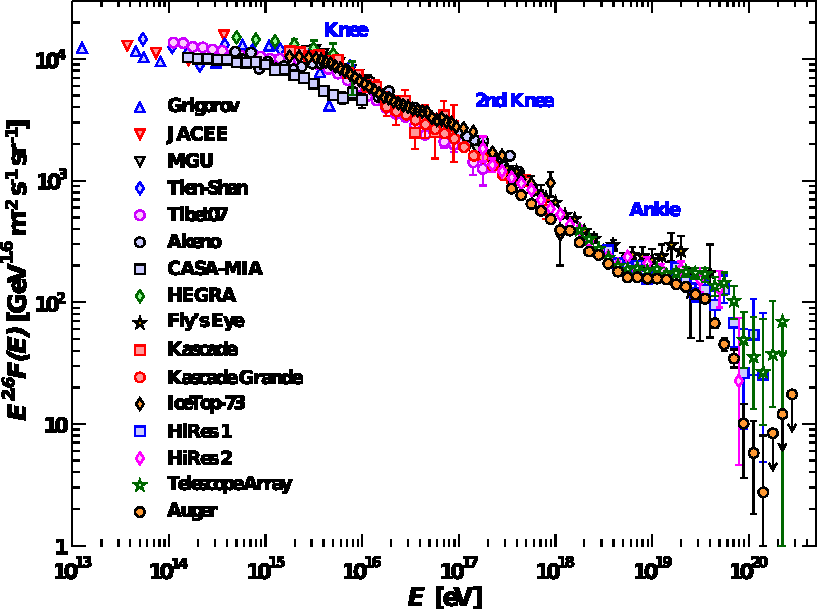
\includegraphics[width=0.8\textwidth]{abbildungen/cr_spectrum_pdg14.pdf}
  \caption{\textbf{Spektrum der kosmischen Strahlung für alle Teilchen aus den Daten von verschiedenen Luftschauerexperimenten.} Aufgetragen ist der differentielle Fluss, gewichtet mit der Energie $E^{2,6}$, gegen die Teilchenenergie pro Nukleon. Gut zu sehen sind das Knie bei etwa $\SI{4e15}{eV}$ und der Knöchel ab $\SI{e18}{eV}$, was die beiden Punkte sind, bei denen sich der Faktor $\gamma$ des Potenzspektrums der kosmischen Strahlung ändert. Mit den neusten experimentellen Daten scheint es auch einen zweites Knie bei $\SI{e17}{eV}$ zu geben. Stand 2014 \ref{ref:pdg14}.}
  \label{fig:cr_spectrum}
\end{figure}

Trifft ein hadronisches Teilchen auf die Atmosphäre, erzeugt es einen hadronischen Luftschauer, bei dem durch hadronische Wechselwirkungen
zu einem Großteil Pionen, aber auch Kaonen entstehen, die durch weitere Zusammenstöße mit Kernen noch mehr Pionen und Kaonen entstehen lassen,
sodass man eine Kaskade von Teilchen erhält. 
Neutrale Pionen zerfallen sehr schnell in zwei Gammaquanten, die durch Paarbildung und Bremmstrahlung elektromagnetische Subschauer entstehen lassen

\begin{equation}
\Pgpz \rightarrow \Pgamma + \Pgamma.
\end{equation}

Geladene Pionen, die ein Drittel der entstehenden Pionen betragen, zerfallen größtenteils in Myonen und Myon-Neutrinos:
\begin{equation}
  \begin{split}
    \Pgpp &\rightarrow \APmuon + \Pgngm  \\
    \Pgpm &\rightarrow \Pmuon + \Pagngm \\
  \end{split}
\label{eq:pipmdecay}
\end{equation}

Der Zerfallskanal in Elektronen und Elektron-Neutrinos ist stark unterdrückt, auch wenn er energetisch günstiger wäre. 
Das liegt daran, dass die schwache Wechselwirkung, der dieser Zerfall unterliegt, eine vektorielle Kraft ist.
Sie koppelt nur an linkshändige Teilchen und rechtshändige Antiteilchen, womit sie stark paritätsverletztend ist.
Damit sind Neutrinos immer linkshändig und Antineutrinos immer rechtshändig, da sie nur schwach wechselwirken und nahezu masselos sind.
Aus der Impulserhaltung folgt, dass das in~\ref{eq:pipmdecay} im Zerfall entstehende Myon bzw. Elektron in die entgegengesetzte Richtung wie
das Neutrino emittiert werden muss. 
Da der Drehimpuls auch erhalten ist, muss zum Beispiel bei einem emittierten rechtshändigen Antineutrino das Elektron bzw. Myon ebenfalls rechtshändig sein. Da Elektronen eine sehr geringe Masse $m_e = \SI{511}{keV}$ haben, treten sie normalerweise meist nur linkshändig auf. Die rechtshändige Komponente ist dagegen stark unterdrückt. Myonen haben eine ungefähr 200-fach höhere Masse, weshalb sie eher rechtshändig auftreten könnten. Daher Zerfallen geladene Pionen meist in Myonen, während der Zerfall in Elektronen nur mit einer Wahrscheinlichkeit von $\SI{1,230+-0,004}{}$~[\ref{ref:pdg14}] auftritt.\\

Freie Myonen haben eine Lebensdauer von 
\begin{equation}
 \tau = \SI{2,197}{\micro\s}. [\ref{ref:pdg14}]
 \label{eq:lebensdauer}
\end{equation}

In dieser Zeit legen sie eine Strecke von $c_0 \cdot \tau \approx \SI{600}{m}$ zurück. 
Da sie normalerweise in mehreren Kilometern Höhe entstehen, würden sie mit einer solchen Lebensdauer im Laborsystem gar nicht bis
auf die Erdorberfläche treffen. Durch ihre hohe Energie haben sie im Laborsystem der Erde durch den Lorentz-Boost eine deutlich höhere Lebensdauer

\begin{equation}
  \tau_E = \gamma\cdot\tau,
\end{equation}
mit dem Lorentz-Faktor $\gamma = \frac{E}{E_0}$. Bei einer Energie von $E = \SI{10}{GeV}$ beträgt da Gamma-Faktor zum Beispiel
\begin{equation}
\gamma \approx \frac{\SI{10}{\giga\electronvolt}}{\SI{140}{\mega\electronvolt}} \approx 71, 
\end{equation}
was die Flugstrecke 71-Fach erhöhen würde, sodass sie normalerweise Problemlos die Erdoberfläche erreichen, wenn man annimmt, dass sie bis dahin nicht wechselwirken. Auf die Wechselwirkung von Myonen mit Materie wird jedoch im nächsten Kapitel eingegangen.\\

% kurz schreiben, dass hochenergetische kosmische teilchen luftschauer erzeugen,
% bei denen durch hadronische wechselwirkungen geladene pionen entstehen, bei deren zerfall myonen entstehen
% vielleicht auch weglassen und erst später beim kapitel zum spin
% lebensdauer von myonen
% evtl. grober wert für den fluss von myonen aus luftschauern


\subsection{Abbremsung von Myonen in Materie}
\label{sec:wwmitmaterie}
Ein weiterer Grund, warum so viele Myonen auf der Erde ankommen, ist, dass sie bei Energien unter GeV-Bereich, anders als Elektronen,
kaum Strahlungsverluste haben, da der Strahlungsverlust durch Bremmstrahlung, der sowas ist wie die Synchrotronstrahlung im Feld der Kerne,
ebenso wie die Synchrotronstrahlung gemäß der Larmor-Formel proportional ist zu $m^{-4}$~\ref{ref:pdg14}. 
Bei mittleren Energien verlieren sie ihre Energie hauptsächlich durch Ionisation. 
Da Myonen somit in der Atmosphäre viel weiter kommen als Elektronen, macht dies möglich, durch die Messung des Verhältnisses der Anzahl von atmosphärischer Elektronen zu Myonen die höhe des Schauermaximums abzuschätzen, da bei einem hohen Schauermaximum die meisten Elektronen auf dem Weg zur Erde absorbiert werden, während die Myonen "`problemlos"' bis an den Erdboden kommen.\\

Myonen werden oft als "`minimal ionizing particles"' (\emph{mips}) bezeichnet, da ihr Energieverlust durch Ionisation bei Energien im GeV-Bereich 
in der Nähe des Minimums der Bethe-Bloch Formel liegt. 
Bei Impulsen im MeV-Bereich~\ref{ref:pdg14} tritt jedoch der Bragg-Peak ein und sie verlieren 
auf kurzem Raum den Großteil ihrer Energie. 
Da sie bei niedrigen Energien nicht mehr dem Lorentz-Boost unterliegen, kann die Messung der Lebensdauer näherungsweise ab dem Zeitpunkt des Einfangs erfolgen. 
Dabei muss dann jedoch beachtet werden, ob man positive oder negative Myonen hat.
Positive Myonen können Elektronen aus den Kernhüllen einfangen und bilden so Myonium, eine wasserstoffähnliches Gebilde, wobei im Gegensatz zum Wasserstoff der Masserschwerpunkt genau zwischen den beiden Teilchen liegt und die effektiven Massen dabei sozusagen halbiert sind.
Die Lebensdauer des Myons bleibt bei diesem Prozess unverändert.
Negative Myonen hingegen können dagegen von den positiven Atomkernen in der K-Schale gefangen werden, da sie durch ihre unterschiedliche 
Teilchenart nicht durch das Pauli-Prinzip von den Elektronen blockiert werden. 
Von da können sie analog zum Elektroneinfang mit einem Proton schwach wechselwirken und dies damit in ein Neutron umwandeln. 
Aufgrund von diesem Prozess haben negative Myonen in Materie eine deutliche niedrigere Lebensdauer, in Kupfer zum Beispiel
\begin{equation}
\tau_{\Pmuon, \mathrm{Kupfer}} = \SI{0,163}{\micro\s}.
\end{equation}
Da man bei der Messung der Lebensdauer dadurch eine Überlagerung zweier Lebensdauern bekommt, ist es geschickt, bei der Messung nur die Ereignisse zu verwenden, bei denen das Signal aus dem Zerfall erst eine Sekunden nach dem Myonen-Trigger kommt, da dann die negativen Myonen größtenteils zerfallen sind.



\subsection{Polarisation von Myonen}
\label{sec:polarisation}
% schwacher wechselwirkung -> vektorielle kraft und paritätsverletzung
% d.h. masselose teilchen immer linkshändig, antiteilchen rechtshändig
% da pion spin 0 hat und neutrino linkshändig ist, muss positron/antimyon auch linkshändig sein
% wegen schwacher ww wären positronen und antimyonen "lieber" rechtshändig
% da positronen kleinere masse haben als anti-muonen (faktor ~200), ist bei ihnen die rechtshändige komponente stärker unterdrückt
% analog für antineutrinos und elektronen/myuonen
% daher zerfall von piplus/piminus hauptsächlich in muonen und nicht in elektronen/positronen

% zerfall in vorwärts und rückwärtsrichtung
% myon erhält dadurch in vorwärts und rückwärtsrichtung unterschiedliche energien im laborsystem bei gleichen pionenenergien
% unterscheidbar durch polarisation



\subsection{Nachweis des Myonenzerfalls}
\label{sec:nachweis}
% die theorie hiervon kann ich auch noch nicht gut (michael)
% aber müsste nicht viel sein


Durch das beim Zerfall emittierte Positron wird der Zerfall gekennzeichnet. Das Spektrum kann differentiell im Raumwinkel $\Omega$ beschrieben werden in der Form

\begin{equation}
\label{eqn:doppeldiffspektrum}
\frac{d^2N}{d\epsilon d\Omega} = \frac{\epsilon^2}{2 \pi} \cdot \left[  (3- 2\epsilon) - P \cdot (1-2\epsilon) \cdot cos(\theta)  \right] = \frac{3 \epsilon^2 - 2 \epsilon^3}{2 \pi} \cdot \left[  1 + P \cdot \frac{2 \epsilon -1}{3 - 2\epsilon} \cdot cos(\theta)  \right] .
\end{equation}

Hierbei ist $P$ die Polarisation, $\theta$ der Winkel zwischen Impuls und Spin des Myons. $\epsilon = E / E_{max}$ ist eine Energie in Einheiten der maximalen Energie $E_{max} = m_{\mu}c^2/2$, die beim Zerfall auf das Myon übertragen werden kann. 

Obige Gleichung lässt sich vereinfacht schreiben als

\begin{equation}
\frac{d^2N}{d\epsilon d\Omega} = a \cdot (1 + b \cdot cos(\theta) ) .
\end{equation}

$b$ läuft von $-\frac{1}{3}$ über $0$ bis $1$. Die Emission des Positrons ist demnach nicht isotrop bezüglich des Spins des $\mu^{+}$. Sie erfolgt bevorzugt in dessen Richtung. Bei höheren Energien ist die Asymmetrie größer. Es existiert eine untere Schwelle für Beobachtung der Positronen. Solche mit zu geringer Energie erreichen den Detektor nicht. 

Wird Gleichung \ref{eqn:doppeldiffspektrum} über $\epsilon$ integriert, erhält man

\begin{equation}
\label{eqn:spektrum}
\frac{dN}{ d\Omega} = k \cdot (1 + A cos(\theta) ).
\end{equation}

$k$ ist ein Konstante, die durch die Schwelle bestimmt wird. $A$ wird als Asymmetrie bezeichnet. Wird über das ganze Spektrum integriert, so ist diese $A=P/3$, für die obere Hälfte erhält man $A = 0.44 P$, der Grenzwert beträgt für hohe Schwellen $A=P$. Bei höheren Schwellen sinkt die Zählrate jedoch ab, sodass zwischen hoher Asymmetrie und Zählrate abgewägt werden muss.

Gleichung \ref{eqn:spektrum} wird über einen endlichen Winkel integriert, um die Winkelverteilung der Positronen zu berücksichtigen. Die Asymmetrie nimmt durch die Mittelung über $\theta$ ab.







\subsection{Präzession von Myonen im Magnetfeld}
\label{sec:prazission}
% gyromagnetische verhältnis gamma, landé-faktor g erklären
% präzission im magnetfeld
% am wichtigsten ist eigentlich nur folgende gleichung:
%\begin{equation}
%g = \frac{\gamma \hbar}{\mu_\mathrm{B}} = \frac{\hbar \omega}{\mu_\mathrm{B}\mathrm{B}}
%\end{equation}

Das Magnetische Moment $\vec{\mu}$ steht mit dem Drehimpuls $\vec{J}$ eines Teilchen in Relation

\begin{equation}
\vec{\mu} = \gamma \cdot \vec{J} .
\end{equation}

Aus der Bewegungsgleichung im Magnetfeld $\vec{B}$

\begin{equation}
\frac{d\vec{J}}{dt} = \vec{\mu} \times \vec{B}
\end{equation}

folgt die Präzesionsfrequens

\begin{equation}
\omega = \gamma \cdot B
\end{equation}

mit dem Betrag des Magnetfeldes $B$ und dem gyromagnetischem Verhältnis 

\begin{equation}
\label{eqn:praez_gyro}
\gamma = \frac{g \mu_B}{\hbar}. 
\end{equation}

Das Bohrsche Magneton $\mu_B$ ist für ein Teilchen der Masse m und der Ladung q

\begin{equation}
\mu_B = \frac{q\hbar}{2 m} .
\end{equation}


Für ein Elektron ergibt dies [\ref{ref:bb}]

\begin{equation}
\mu_B (Elektron) = \SI{9.273e-24}{ J/T } .
\end{equation}

Für das schwerere Myon beträgt es [\ref{ref:bb}]

\begin{equation}
\mu_B (Elektron) = \SI{4.485e-26}{ J/T } .
\end{equation} 


Der dimensionslose Faktor $g$ wird als \textbf{Landé-faktor} bezwichnet. Für den Bahndrehimpuls ist er genau gleich eins. Für den Spin ist er 2 + Korrekturen höherer Ordnung. Nach Gleichung \ref{eqn:praez_gyro} lässt er sich berechnen mit

\begin{equation}
g = \frac{\gamma \hbar}{\mu_B} = \frac{\hbar \omega}{\mu_B B} .
\end{equation}


\subsection{Messprinzip}
\label{sec:messprinzip}
% zerfall von myonen erfolgt exponentialgesetz
% wie misst man präzission?
% -> angelegtes magnetfeld
% formeln...

\subsubsection*{Messung der mittleren Lebensdauer}

Die Messung startet mit der Registrierung der Abbremsung eines Myons im Detektor. Durch den Zerfall entsteht ein Positron, dessen Auftreten die Messung stoppt. Da es sich um einen Zerfall handelt, kann man für viele beobachtete Myonen ein Exponentialgesetz ansetzen:

\begin{equation}
\label{eqn:messprinzip-zerfall}
N(T) = N_0 \cdot exp(-t / \tau) .
\end{equation} 
	
$N_0$ ist die Gesamtzahl der im Detektor gestoppten Myonen während der Messzeit, $N$ die Anzahl der beobachteten Zerfälle.
Die mittlere Lebensdauer $\tau$ kann man bestimmen, auch ohne die Energie und Richtung der Myonen zu betrachten. 

\subsubsection*{Messung der Präzessionsfrequenz}


Über das Stopptarget wird ein Magnetfeld transversal zur Einfallsrichtung der Myonen gelegt, in diese präzedieren.
Indem nur in eine bestimmte Richtung emittierte Positronen gemessen werden, ist die Zählrate mit der Präzessionsfrequenz moduliert. Ist der Spin der Myonen antiparallel zur Richtung, ist er am geringsten, bei parallel gerichtetem am höchsten.


Gleichungen \ref{eqn:spektrum} und \ref{eqn:messprinzip-zerfall}
lassen sich zusammenfassen zu

\begin{equation}
N(t) = K \cdot exp(- \frac{t}{\tau}) \cdot \left[ 1 + \overline{A} \cdot cos(\omega t + \delta) \right] .
\end{equation}

Die Exponentialfunktion entstammt dem Zerfallsgesetz aus Gleichung \ref{eqn:messprinzip-zerfall}, der Term in der eckigen Klammer beschreibt die Modulation durch Präzession.
$\overline{A}$ ist die, über die Geometrie des Detektors gemittelte, Asymmetrie. Diese ist aufgrund der Depolarisation der $\mu^{+}$ zeitabhängig und folgt einem Exponentialgesetz

\begin{equation}
\overline{A} = \overline{A}_0 \cdot exp(- \frac{t}{ T_R }) .
\end{equation}

In Kupfer kann sie jedoch als konstant angenommen werden. $T_R$ bezeichnet die Relaxationszeit.
	
\clearpage

\section{Versuchsaufbau und Durchführung}
% von oben nach unten: Szinti 1, Szinti 2, Kupferabsorber in Magnetfeld, Szinti 3
% Koinzindenz und Veto-Schaltung erklären: 
% D.h. Wir nehmen nur die Ereignisse, wo 1 und 2 gleichzeitig ausschlagen (Koinzindenz) und 3 NICHT ausschlägt (Veto bzw Antikoinzindenz)
% erklären was ein diskriminator in der analog-digitalwandlung ist und wie die schwelle (trigger) eingestellt werden muss:
% trigger muss so sein, dass untergrund unterdrückt wird und man nur hauptsignal sieht
% zu hoher trigger verringer unnötig statistik
% trigger für veto (szinti 3) lieber etwas niedriger als zu hoch, damit man keine falschen ereignisse aufnimmt
% was ist ein TAC (zeit-amplituden-converter) und zeiteichung ?

In Abbildung \ref{fig:aufbau_skizze} ist eine Skizze des Versuchsaufbaus gezeigt. Drei Szintillatorplatten, mit einer Dicke von $\SI{2.5}{cm}$, sind waagerecht übereinandergelegt. Zwischen dem zweiten und dritten befindet sich eine ebenso dicke Kupferplatte, welches die $\mu^{+}$ stoppt. 
Signale aus den Szintillatoren werden mit einem Photomultiplier (PM) verstärkt und in die Koinzidenz geschickt.
Ein gestopptes Myon hat die Signatur $1 + 2 + \overline{3}$, also eine Koinzidenz der oberen Szintillatoren und eine Antikoinzidenz des unteren. Damit wird die Messsung begonnen. Die Messung wird beendet, wenn ein Positron detektiert wird. Dieses kann in Richtung des Szintillators 2, oder 3 emittiert werden. Das Stoppsignal auszusenden, wenn eines der beiden Szintillatoren ein Signal aussendet ist jedoch nicht optimal, da zufällige Stopps aufgrund von Hintergrundstrahlung auftreten. Am besten eignet sich eine Signatur $1 + 2 + \overline{3}$. Die Zählrate ist hier jedoch abgeschwächt.  


\begin{figure}[tb!]
  \centering
  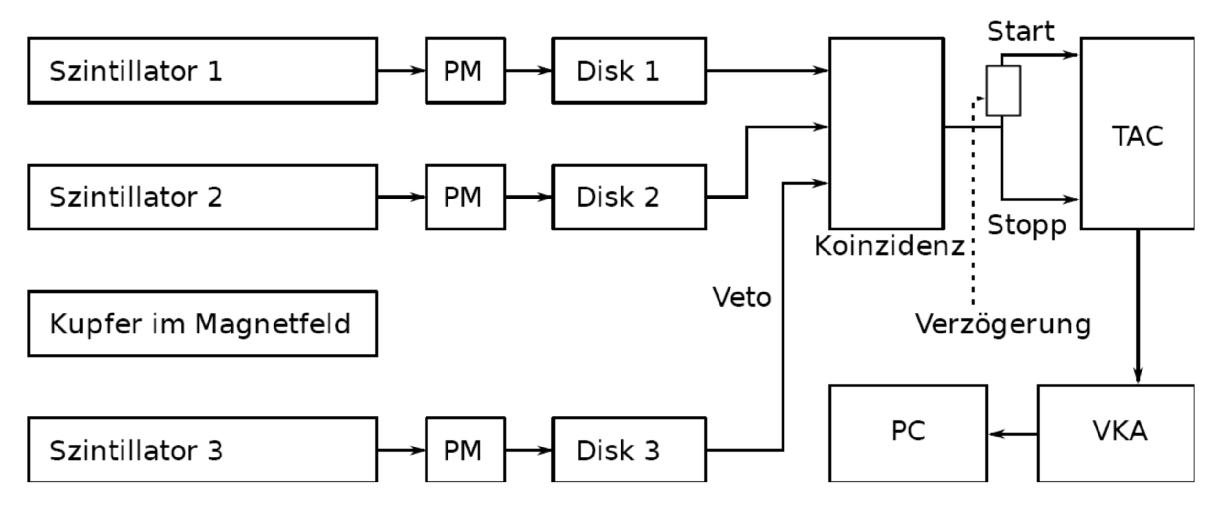
\includegraphics[width=0.8\textwidth]{abbildungen/aufbau_skizze.png}
  \caption{\textbf{Skizze des Versuchsaufbaus.} 
  \\ 
  Drei Kunstoffszintillatoren und eine Kupferplatte mit einer Dicke von jeweils $\SI{2.5}{cm}$ sind übereinander angeordnet. Die Kupferplatte befindet sich zwischen dem 2. und 3. Szintillator. Das Signal aus den Szintillatoren wird mit Photomultpliern (\textbf{PM}) verstärkt. Bei den definierten Signatur wird von der Koinzidenz ein Signal für den Start, bzw. Stopp der Messung gegeben. Das Startsignal wird um einige Nanosekunden verzögert, damit der Time to Amplitude Converter (\textbf{TAC}) das Signal verarbeiten kann. Über einen Vielkanalanalysator (\textbf{VKA}) wird das Signal an einem Rechner (\textbf{PC}) analysiert.
  \\Quelle: [\ref{ref:bb}]}
  \label{fig:aufbau_skizze}
\end{figure}

Der Time to Amplitude Converter (TAC) kann Signale nicht verarbeiten, wenn diese gleichzeitig eintreffen. Da Start- und Stoppsignal die selbe Signatur haben, ist die der Fall. 
Daher wird das Startsignal um einige Nanosekunden verzögert. 
Das verzögerte Startsignal eines Myons startet den Zähler, wird aber nicht von dessen Stoppsignal gestoppt. Das nächste Stoppsignal kommt erst bei dem nächsten Myon. Hier liegt das Stoppsignal aufgrund der Verzögerung schneller an, als dessen Startsignal. Seit $T_{1-2}$ die Zeit, die zwischen dem Eintreffen der beiden Myonen vergangen ist, $\tau_1$ und $\tau_2$ die Lebensdauern der beiden Myonen und $\delta t$ die Verzögerung am Startsignal. 

Ohne Verzögerung und mit einem entsprechend schnellen Detektor würde ein Startsignal kommen, gefolgt von dem Stoppsignal für jedes Myon. Man würde die Lebensdauer also direkt messen, was aber hier nicht möglich ist. Stattdessen misst man die Zeit von dem verzögertem Startsignal des ersten bis zu dem Stoppsignal des zweiten Myons. Die gemessene Zeit ist also

\begin{equation}
t = T_{1-2} - \tau_2 .
\end{equation}

Das Startsignal des zweiten Myons wird ignoriert, denn der TAC benötigt einige Microsekunden, um das analoge Signal zu erzeugen.



\subsection{Zusätzliche Aufgaben}

\begin{itemize}
\item a) Einstellung der Schwellen an den Diskriminatoren
\item b) Zeiteichung des Zeit-zu-Amplituden-Konverters (TAC)
\end{itemize}



\clearpage
\section{Quellen}
\begin{enumerate}
\item \emph{Einführung in das Kernphysikalische Praktikum} von F. K. Schmidt, 
  Überarbeitung von J. Wolf, Ausgabe September 2009. \label{ref:bb}
\item K.A. Olive et al. (Particle Data Group), Chin. Phys. C, 38, 090001 (2014). \label{ref:pdg14}
\end{enumerate}



\end{document}
